Referential games are confined interactive reasoning tasks used to
study pragmatic inference in a controlled environment
\cite{StillerGoodman2011:Ad-Hoc-Scalar-I,Frank,Degen}. A referential game
consists of a set of objects called a \textit{context}. For example, a
context might contain different shapes of different colors in various
arrangements, such as shown in Figure~\ref{context}.  The speaker in
the game is asked to refer to one of the objects (the \emph{target})
by uttering an expression (typically a single word denoting a feature,
i.e., color or shape, of the target) to the listener. The listener,
who does not know which object is the target, needs to recover the
target based on the speaker's choice of expression.

\begin{figure}[h] 
  \centering \subfigure[Example context: green square and circle, and
  blue circle.]{\label{context}
  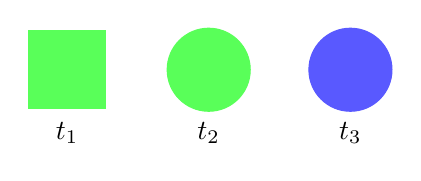
\begin{tikzpicture}
     \path (-1.8, 0) node [shape=rectangle, draw=green!65 ,fill= green!65 ,minimum size=28]{}
           ( 0, 0) node  [shape=circle, draw=green!65, fill= green!65,minimum size=30] {}
           ( 1.8, 0) node [shape=circle, draw=blue!65, fill=blue!65  ,minimum size=30] {}
           ( -1.8, -0.8) node {$t_{1}$}
           ( -0.0, -0.8) node {$t_{2}$}
           (  1.8, -0.8) node {$t_{3}$}
     ;
           
  \end{tikzpicture}
}\hspace{5mm} \subfigure[Vocabulary and truth table]{\label{VaTT}
  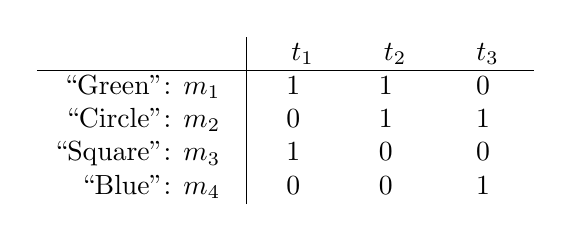
\begin{tikzpicture}
     \path (0,0) node[] 
     {\begin{tabular}{r|ccc}
                         & \quad $t_{1}$\ \  &\quad $t_{2}$\ \  &\quad $t_{3}$ \ \   \\
    \hline
   ``Green'':  $m_{1}$ \quad  &  $1$        &   $1$       & $0$      \\
   ``Circle'': $m_{2}$  \quad &  $0$        &   $1$       & $1$      \\ 
   ``Square'': $m_3$ \quad    &  $1$      &   $0$       & $0$      \\
   ``Blue'':   $m_4$  \quad  &  $0$        &   $0$       & $1$     
     \end{tabular}
     } ;
  \end{tikzpicture}
  }
  \caption{A simple referential game, as used in \cite{Frank}}
\end{figure}


Let us first try to play this game ourselves, to get a better sense of
what it is about and why it is relevant to human pragmatic
reasoning. For simplicity let us assume that the utterances that the
speaker is allowed to use are from a \emph{vocabulary} which is
commonly known between the speaker and the listener. The content of
the vocabulary and the (truth-conditional/literal) meaning of each
word are shown in Figure \ref{VaTT}. Suppose we play as the speaker
and the target is $t_1$, the green square. We can either use
``Square'' or ``Green'' to truthfully refer to it, but it seems more
prudent to use ``Square'', as there is only one square in the context
and thus the listener can easily identify it, whereas there are two
green objects, which makes ``Green'' ambiguous. In terms of the
Gricean \emph{Maxim of Quantity}, we should use ``Square'' because it
is more informative than ``Green'' in the given context; the surplus
informativity moreover seems relevant. Similarly, we should use
``Blue'' to refer to $t_3$, the blue circle. However, using ``Blue''
to refer to the blue circle might intuitively sound a little
unnatural, as color terms are usually used as adjectives\footnote{They
  are used as nouns mostly to refer to the colors themselves.}, while
we usually use nouns to refer to concrete objects. This inclination
becomes more evident when we want to refer to $t_2$, the green
circle. While ``Green'' and ``Circle'' are equally ambiguous in this
case, we might nevertheless prefer the latter.

Now let us turn to play as the listener. If we hear ``Square'' or
``Blue'', we easily know the intended referent as there is no
ambiguity, but what if we hear ``Circle'' (or ``Green'')? There are
two circles in the context that we need to choose from. On the one
hand, the blue circle, having the unique color in the context, seems
to be perceptually dominant and thus easily captures our attention. On
the other hand, from the previous analysis we know that if the blue
circle were the intended referent, the speaker could have chosen
``Blue'' which is not ambiguous and thus more informative. Hence the
listener needs to balance two sources of information, i.e., the
(presumably subconscious) perceptual salience of different objects and
the rational expectation of the likelihood of the speaker making the
utterance for each object. 

To test these intuitions, Frank \& Goodman recruited 745 US
participants via Amazon's Mechanical Turk to take part in a one-shot
referential game, either as the speaker or the listener \cite{Frank}.
The context of the game always consisted of three objects (e.g.,
Figure~\ref{context}).  Each object had three features: color (red,
blue, or green), shape (circle, square, or cloud), and texture (solid,
or polka-dot, or striped).  Every context had one feature fixed for
all objects and the other two features systematically varied.  The
objects were randomly permuted and the target object was randomly
assigned.  Depending on how many objects shared the same value of a
feature with the target, contexts were classified into 7 categories:
1/1, 1/2 (the target's first feature is unique, and there is another
object sharing the same value of the second feature with the target),
1/3, 2/2 with the same object sharing both features with the target
(which means there is another object identical to the target), 2/2
with different objects sharing the features (such as in
Fig.~\ref{context}), 2/3 and 3/3. The speakers were asked to choose a
feature to refer to the target object.\footnote{More accurately,
  participants were ask to \emph{bet} on features and referents. We
  will discuss this design choice when contrasting it with our own
  replication experiment in Section~\ref{sec:experiment}.}  In order
to measure the perceptual salience, some of the listeners were told
that the speaker was using a language that they did not understand and
then they were asked to guess the intended referent.  Other listeners
were told a feature of the target and asked to choose the intended
referent.

The result of the experiment showed that speakers generally followed
Grice's Maxim of Quantity, i.e., they tried to be informative by
choosing the most unique feature of the target, and that listeners
were influenced by both the perceptual salience and the
informativeness of the utterance that the speaker produced. However,
the data, being quantitative in nature, cannot be fully explained by a
classical qualitative Gricean account of scalar implicatures, so that
a major challenge in terms of formal modeling becomes how to quantify
notions such as informativeness and perceptual salience, and how these
should be integrated to yield qualitative predictions.

The rational speech-act model (RSA) model addresses these issues by
using information-theoretic concepts to measure informativeness and
Bayesian inference to integrate different sources of information
\cite{Frank2009,Frank,Bergen2012,GoodmanStuhlmuller2013:Knowledge-and-I}. In
order to measure the informativeness of an utterance, the RSA model
starts with the literal listener who upon receiving an utterance $m$
does a conditioning on its literal meaning:
\begin{equation}\label{Bayesian_literal}
\rho_0(t \mid m) = \mathcal{U}(t\mid \intp{m}) ,
\end{equation}
where $\mathcal{U}$ is a uniform distribution over all the possible
referents. The informativeness of utterance $m$ for the intended
referent $t$ can be measured as the negative Kullback-Leibler
divergence of the induced literal listener's belief $\rho_0$ from the
speaker's own belief $\delta_t$:
\begin{equation} \label{Bayesian_sender_informativeness}
\mbox{Info}(m,t)=-\mbox{KL}(\delta_t \| \rho_0)=-\sum_{t'}\delta_t(t')\log\left(\frac{\delta_t(t')}{\rho_0(t')}\right),
\end{equation}
where $\delta_t$ is a delta distribution with all probability mass on
target object $t$, as the speaker knows her intended referent:
\begin{equation} \label{Bayesian_sender_delta}
\delta_t(t')=\left\{ \begin{array}{ll}
1 & \mbox{if } t' = t \\
0 & \mbox{otherwise}
\end{array}\right. \enspace .
\end{equation}

The speaker acts sub-optimally by choosing the utterance that soft-maximizes her expected utility, which is defined as the informativeness of the utterance subtracted by its cost:
\begin{equation} \label{Bayesian_sender_softmax}
\sigma(m \mid t) \propto \exp(\lambda_\mathrm{S}\cdot \mbox{U}(m,t))=\exp(\lambda_\mathrm{S} \cdot (\mbox{Info}(m,t)-\mbox{Cost}(m))),
\end{equation}
where $\lambda_\mathrm{S}$ is a parameter measuring the speaker's
degree of rationality, i.e., to what extent the speaker sticks to the
strict optimum.\footnote{Mathematically, it can be shown that when $\lambda_\mathrm{S}=0$, $\sigma(m \mid t)$ is uniformly distributed over all messages, meaning that the speaker just randomly selects one of the messages without any optimality consideration. 
On the other hand, when $\lambda_\mathrm{S}\rightarrow \infty$, 
$\sigma(m \mid t)$ is non-zero only when $m$ yields the maximal utility, 
meaning that the speaker only selects the strictly optimal option(s).
This rule is widely used in the AI literature (e.g., \cite{Sutton1998RL}) and 
is also known as \emph{exponential choice rule}.}
The cost term is used to encode preference in
different utterances, be it about the utterances' lengths or syntactic
categories.

From (\ref{Bayesian_literal})-(\ref{Bayesian_sender_softmax}) we
obtain the speaker's production rule:\footnote{Note that we can further
  simplify (\ref{Bayesian_speaker}) as follows:
  $\exp(\lambda_\mathrm{S} \cdot (\log \mathcal{U}(t\mid
  \intp{m})-\mbox{Cost}(m))) =\exp(\lambda_\mathrm{S} \log
  \mathcal{U}(t\mid \intp{m}) \cdot \exp(-\lambda_\mathrm{S}\cdot
  \mbox{Cost}(m)) =(\mathcal{U}(t\mid
  \intp{m}))^{\lambda_\mathrm{S}}\cdot \exp(-\lambda_\mathrm{S}\cdot
  \mbox{Cost}(m))$. Incidentally, if we do not take costs into
  account, i.e., let $\mbox{Cost}(m) = 0$, then
  (\ref{Bayesian_speaker}) reduces to $\sigma(m \mid t) \propto
  (\mathcal{U}(t\mid \intp{m}))^{\lambda_\mathrm{S}}$, which is
  effectively a \emph{power rule} that soft-maximizes
  $\mathcal{U}(t\mid \intp{m})$. In this respect
  (\ref{Bayesian_speaker}) can be seen as an action-oriented speaker
  model (the exact definition of which will be given in the next
  section) equipped with a different kind of soft-max rule. However,
  we note that this is a mere technical coincidence, and as a first
  step, throughout this paper we only consider the exponential rule as
  the soft-max rule. \cite{Worthy2008ratio} provides a detailed
  discussion and empirical analyses on the differences between the
  exponential and power rules.}

\begin{equation} \label{Bayesian_speaker}
\sigma(m \mid t) \propto \exp(\lambda_\mathrm{S} \cdot (\log \mathcal{U}(t\mid \intp{m})-\mbox{Cost}(m))) \enspace .
\end{equation}

The pragmatic listener in the RSA model, upon receiving the utterance
$m$, performs a Bayesian update on his prior belief $\mathcal{S}(t)$
by using an estimate of the speaker's behavior
(\ref{Bayesian_speaker}):
\begin{equation} \label{Bayesian_rec_update}
\rho(t \mid m) \propto \mathcal{S}(t)\cdot \sigma(m \mid t) \enspace .  
\end{equation}
Bayes' rule naturally integrates the perceptual salience of each
object, which is treated as the prior $\mathcal{S}(t)$ and can be
empirically measured, with listener's expectation of the speaker being
informative, which is incorporated as the likelihood, thus addressing
the previously mentioned challenge of balancing different sources of
information. Setting $\lambda=1$ and $\mbox{Cost}(m)=0$ for all $m$,
\cite{Frank} obtained a highly significant correlation between the
model prediction and their experiment data on actual speaker and
listener behavior gathered from referential games of varying
complexity.


%%% Local Variables: 
%%% mode: latex
%%% TeX-master: "main"
%%% TeX-PDF-mode: t
%%% End: